% epilogue.tex
%
% Author       : James Mnatzaganian
% Contact      : http://techtorials.me
% Date Created : 08/27/15
%
% Description  : The epilogue used by "thesis.tex".
%
% Copyright (c) 2015 James Mnatzaganian

% NOTE: All filler text has "TODO" written. This must be removed in the final copy!

% Bibliography
\bibliography{thesis}
\bibliographystyle{plain}

% Glossary
\printglossary[type=main]

\begin{appendices}
	
	\chapter{SVM Feature Dependency Experiment}
	\label{sec:svm_app}
	
	
	One additional way to confirm the dependencies highlighted through drop in histogram intersection and conditional entropy is to test with a simple model for separation. To do so, a SVM with the RBF Kernel function was trained using all unique permutations of features. The model was given 1 to $n-1$ features as conditioners and an expected output feature for all possible input-output pairs. 
	
	To further prove that the dependencies identified by the GAN exist, a SVM was fit to the $1|2$-combination distributions for each of the target machines from the CPTC'17 dataset. The accuracy of this fit was tabulated for all four victim IP addresses tested in Table \ref{table:svm_accuracy}.
	
	\begin{table}[!htbp]
		\caption{SVM Prediction Accuracy For 3-Combination Feature Values Assorted Victim IPs}
		\label{table:svm_accuracy}
		\centering
		\begin{tabular}{l|cccc}
			\multicolumn{1}{l|}{} & \multicolumn{4}{c|}{\textbf{Machine IP Address}} \\
			\multicolumn{1}{l|}{\textbf{Prediction{\given}Features}} & \multicolumn{1}{l}{\textbf{10.0.0.100}} & \multicolumn{1}{l}{\textbf{10.0.0.27}} & \multicolumn{1}{l}{\textbf{10.0.0.22}} & \multicolumn{1}{l|}{\textbf{10.0.99.143}} \\ \hline
			\multicolumn{1}{l|}{\textbf{D{\given}A,T}} & \multicolumn{1}{c|}{0.958} & \multicolumn{1}{c|}{0.591} & \multicolumn{1}{c|}{0.949} & \multicolumn{1}{c|}{0.908} \\
			\multicolumn{1}{l|}{\textbf{D{\given}A,S}} & \multicolumn{1}{c|}{0.962} & \multicolumn{1}{c|}{0.616} & \multicolumn{1}{c|}{0.970} & \multicolumn{1}{c|}{0.977} \\
			\multicolumn{1}{l|}{\textbf{D{\given}S,T}} & \multicolumn{1}{c|}{0.790} & \multicolumn{1}{c|}{0.541} & \multicolumn{1}{c|}{0.879} & \multicolumn{1}{c|}{0.794} \\
			\multicolumn{1}{l|}{\textbf{A{\given}D,T}} & \multicolumn{1}{c|}{0.911} & \multicolumn{1}{c|}{0.490} & \multicolumn{1}{c|}{0.929} & \multicolumn{1}{c|}{0.472} \\
			\multicolumn{1}{l|}{\textbf{A{\given}S,D}} & \multicolumn{1}{c|}{0.852} & \multicolumn{1}{c|}{0.516} & \multicolumn{1}{c|}{0.889} & \multicolumn{1}{c|}{0.486} \\
			\multicolumn{1}{l|}{\textbf{A{\given}S,T}} & \multicolumn{1}{c|}{0.749} & \multicolumn{1}{c|}{0.440} & \multicolumn{1}{c|}{0.811} & \multicolumn{1}{c|}{0.344} \\
			\multicolumn{1}{l|}{\textbf{S{\given}A,T}} & \multicolumn{1}{c|}{0.719} & \multicolumn{1}{c|}{0.742} & \multicolumn{1}{c|}{0.539} & \multicolumn{1}{c|}{0.702} \\
			\multicolumn{1}{l|}{\textbf{S{\given}D,T}} & \multicolumn{1}{c|}{0.736} & \multicolumn{1}{c|}{0.814} & \multicolumn{1}{c|}{0.525} & \multicolumn{1}{c|}{0.729} \\
			\multicolumn{1}{l|}{\textbf{S{\given}A,D}} & \multicolumn{1}{c|}{0.962} & \multicolumn{1}{c|}{0.616} & \multicolumn{1}{c|}{0.970} & \multicolumn{1}{c|}{0.977} \\
			\multicolumn{1}{l|}{\textbf{T{\given}A,S}} & \multicolumn{1}{c|}{0.411} & \multicolumn{1}{c|}{0.387} & \multicolumn{1}{c|}{0.215} & \multicolumn{1}{c|}{0.459} \\
			\multicolumn{1}{l|}{\textbf{T{\given}S,D}} & \multicolumn{1}{c|}{0.408} & \multicolumn{1}{c|}{0.424} & \multicolumn{1}{c|}{0.161} & \multicolumn{1}{c|}{0.514} \\
			\multicolumn{1}{l|}{\textbf{T{\given}A,D}} & \multicolumn{1}{c|}{0.178} & \multicolumn{1}{c|}{0.208} & \multicolumn{1}{c|}{0.189} & \multicolumn{1}{c|}{0.436} \\
		\end{tabular}
	\end{table}
	
	Note that the order of the combinations is the same as that given in Table \ref{tab:ce} and held constant for all victim IPs. Though some general trends exist, such as alert signature and destination port category being poor predictors of timestamp, there is variation between the different victims. Fig. \ref{fig:entropy_v_accuracy} shows that regardless of what feature dependencies exist for a given victim there is a strong negative correlation between accuracy of an SVM predictor and the conditional entropy.
	
	\begin{figure}[!htbp]
		\centering
		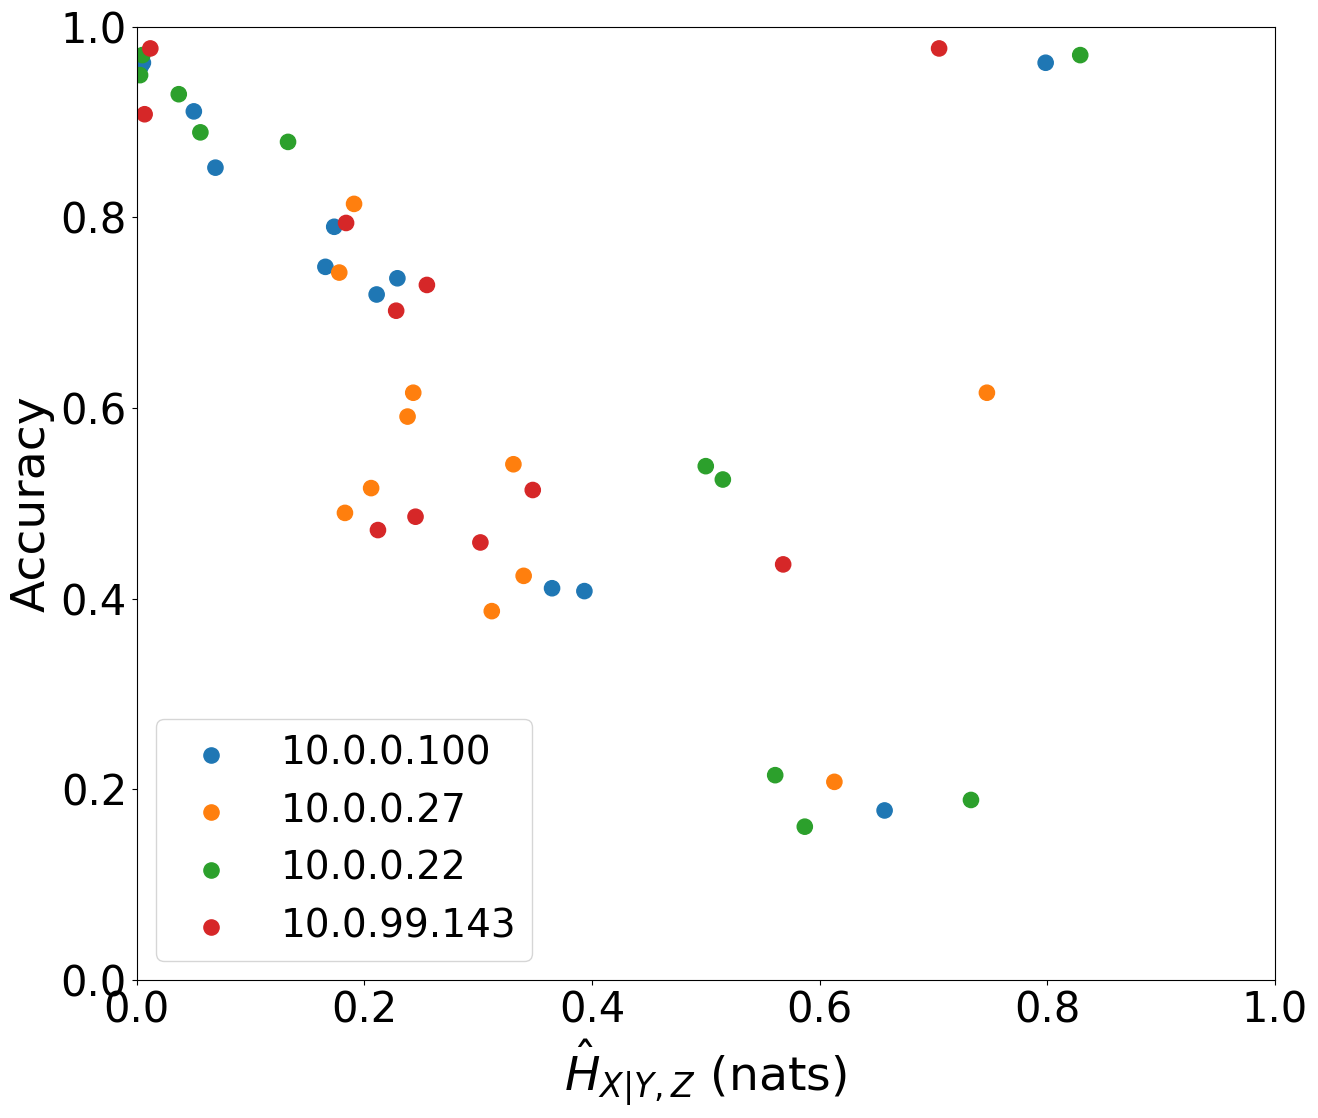
\includegraphics[width=.75\textwidth]{entropy_vs_accuracy.png}
		\caption{SVM Accuracy Plotted Against Conditional Entropy}
		\label{fig:entropy_v_accuracy}
	\end{figure}
	
	
\chapter{Alert Dependency Plots}
	\label{sec:depend_app}
	
	\begin{figure}[!htbp]
		\centering
		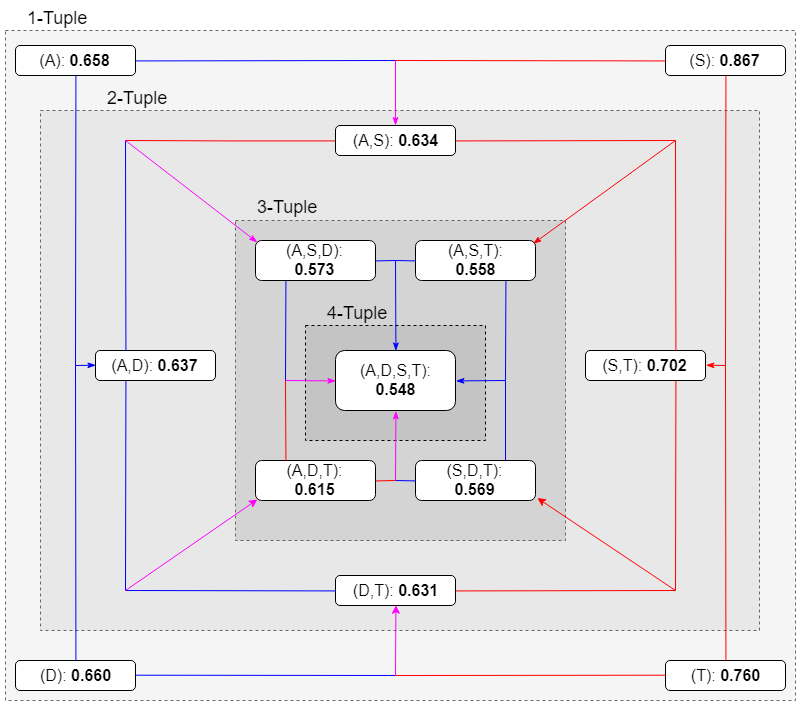
\includegraphics[width=.75\textwidth]{WGAN_22}
		\caption{
			Target 10.0.0.22 Alert Dependency Graph: WGAN-GP Result
		}
		\label{fig:alert_depend_2}
	\end{figure}
	
	\begin{figure}[!htbp]
		\centering
		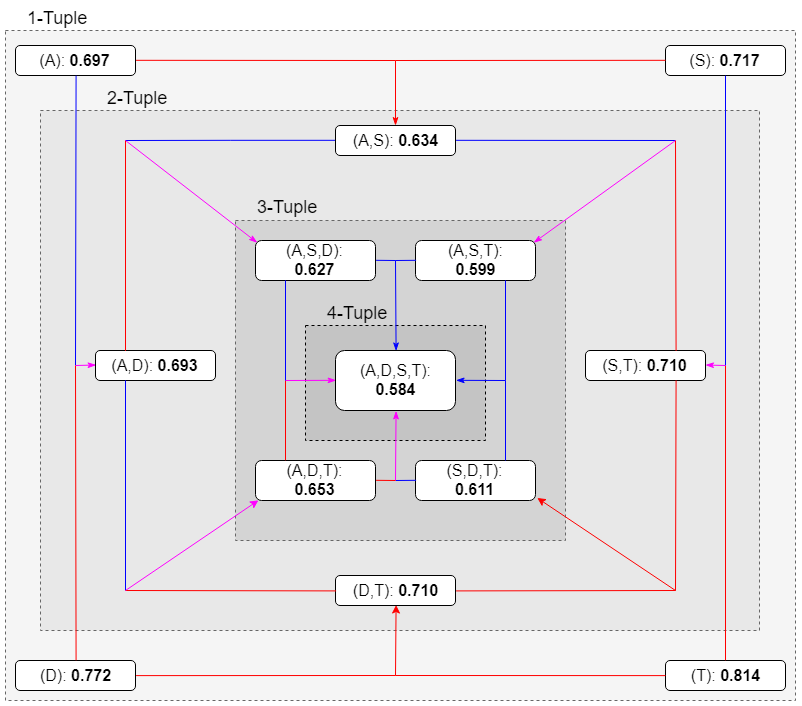
\includegraphics[width=.75\textwidth]{WGAN_100}
		\caption{
			Target 10.0.0.100 Alert Dependency Graph: WGAN-GP Result
		}
		\label{fig:alert_depend_3}
	\end{figure}
	
	\begin{figure}[!htbp]
		\centering
		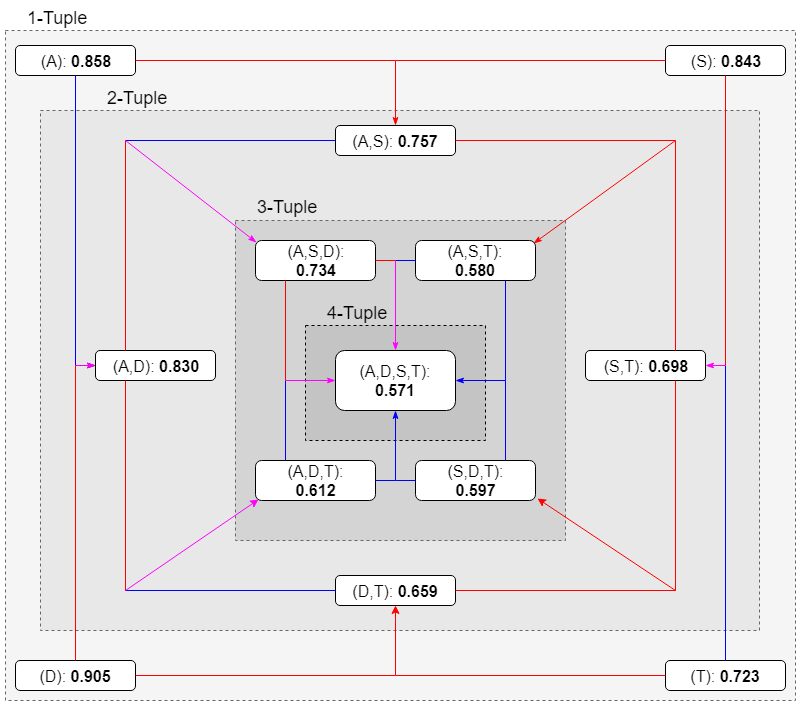
\includegraphics[width=.75\textwidth]{WGAN_143}
		\caption{
			Target 10.0.99.143 Alert Dependency Graph: WGAN-GP Result 
		}
		\label{fig:alert_depend_4}
	\end{figure}

	\begin{figure}[!htbp]
		\centering
		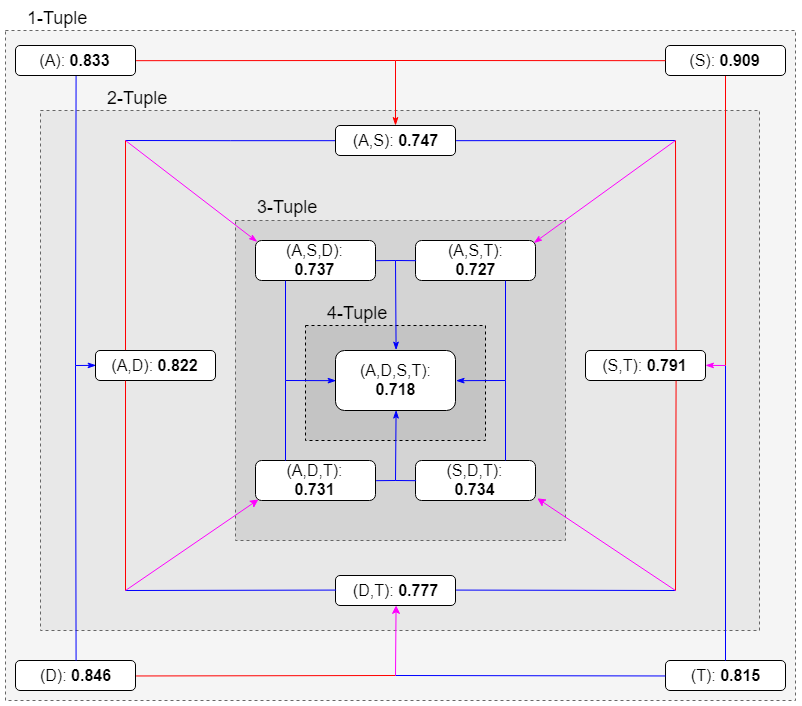
\includegraphics[width=.75\textwidth]{GPMI_22}
		\caption{
			Target 10.0.0.22 Alert Dependency Graph: WGAN-GPMI Result
		}
		\label{fig:alert_depend_6}
	\end{figure}
	
	\begin{figure}[!htbp]
		\centering
		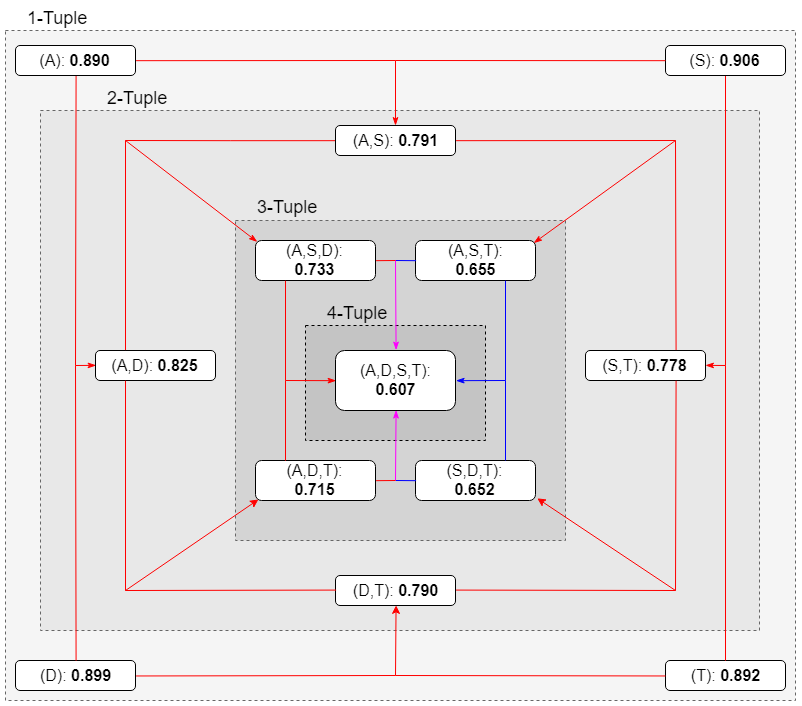
\includegraphics[width=.75\textwidth]{GPMI_100}
		\caption{
			Target 10.0.0.100 Alert Dependency Graph: WGAN-GPMI Result
		}
		\label{fig:alert_depend_7}
	\end{figure}
	
	\begin{figure}[!htbp]
		\centering
		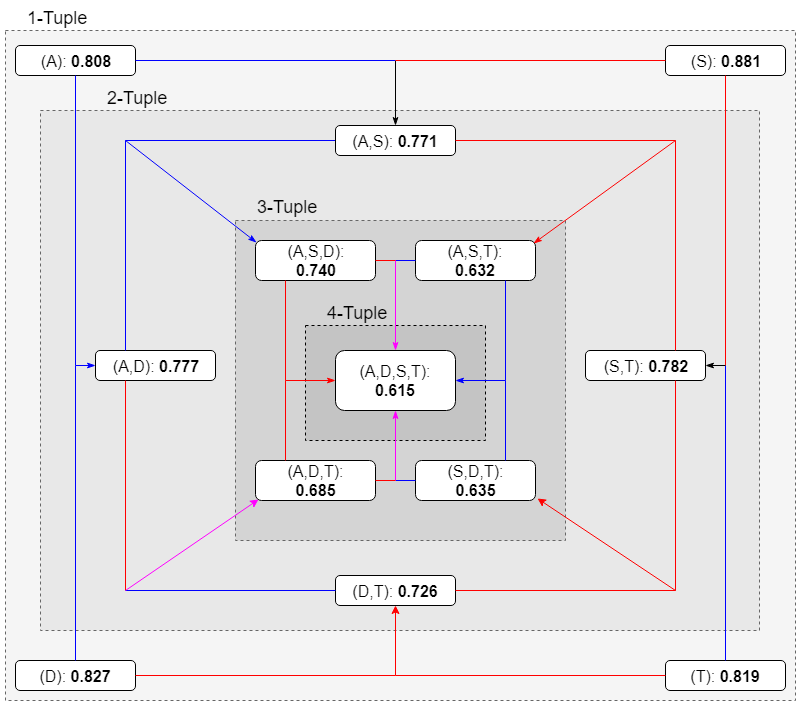
\includegraphics[width=.75\textwidth]{GPMI_143}
		\caption{
			Target 10.0.99.143 Alert Dependency Graph: WGAN-GPMI Result 
		}
		\label{fig:alert_depend_8}
	\end{figure}

	\chapter{Alert Dependency Plots}
	\label{sec:iana_app}
	The Common Port Services listing provided by IANA is available at the following url:
	\href{https://www.iana.org/assignments/service-names-port-numbers/service-names-port-numbers.xhtml}{https://www.iana.org/assignments/service-names-port-numbers/service-names-port-numbers.xhtml}
	Note that these mappings are periodically updated and are only common mappings/suggestions. Individual corporations may opt to configure their own service mapping. 


\end{appendices}